% $Id: anhang.tex,v 1.14 2010/08/10 08:17:41 baum Exp $
% Tag $Name: tinyheb-1-6-3 $

% Copyright (C) 2004 - 2009 Thomas Baum <thomas.baum@arcor.de>
% Thomas Baum, 42719 Solingen, Germany

% This program is free software; you can redistribute it and/or modify
% it under the terms of the GNU General Public License as published by
% the Free Software Foundation; either version 2 of the License, or
% (at your option) any later version.

% This program is distributed in the hope that it will be useful,
% but WITHOUT ANY WARRANTY; without even the implied warranty of
% MERCHANTABILITY or FITNESS FOR A PARTICULAR PURPOSE.  See the
% GNU General Public License for more details.

% You should have received a copy of the GNU General Public License
% along with this program; if not, write to the Free Software
% Foundation, Inc., 59 Temple Place - Suite 330, Boston, MA 02111-1307, USA.



\appendix
\chapter{Anhang}

\section{Anmeldung zum E-Mail Verfahren\label{anhang:elekrech}}
\index{Datenaustausch!Anmeldung}
Hier findet sich die Beschreibung, was zu tun ist, um Rechnungen per
E-Mail zu verschicken. Der hier beschriebene Weg ist vom Autor selbst
beschritten worden. Dies wird ausdrücklich erwähnt, weil sich im Internet
an unterschiedlichsten Stellen Anweisungen finden, was zu tun ist und
wie viel es kostet. Diese Beschreibungen sind oft nicht korrekt, insb.
ist es nicht notwendig Geld für eine Zulassung zum Datenaustausch
auszugeben.

Wie immer im Leben führen viele Wege nach Rom und genau so ist es auch
mit der Zulassung zum Datenaustausch. 

\paragraph{Weg 1}
Auf der Anmeldeseite der ITSG \cite{itsg_email_anmeldung} findet sich
seit März 2006 ein Hinweis, dass nach dem Beschluss der Technischen
Arbeitsgruppe eine Anmeldung zum Praxisverfahren für Leistungserbringer
und Arbeitgeber nicht mehr erforderlich ist und aus diesem Grund die
entsprechenden Anmeldeformulare auf dieser Internet-Seite nicht mehr zu
Verfügung stehen.

Das ist auch gut so, weil eine Anmeldung über dieses Formular nicht 
funktionierte. Daher geht man besser Weg 2:

\paragraph{Weg 2}
Dieser Weg führt einen zu den verschiedenen Datenannahmestellen, bzw.
den einzelnen Krankenkassen und den in \cite{datenaustausch302} genannten
Ansprechpartnern. Welche das sind, ist in Tabelle \ref{krankenkassen302}
aufgeführt, unbedingt anmelden muss man sich beim VdAK.

\paragraph{}

\bottomcaption{Krankenkassen und Ansprechpartner\label{krankenkassen302}}
\tablehead
{\hline \bfseries Krankenkassen&\bfseries Anmeldung und Ansprechpartner\\ \hline}

\tabletail
{\hline \multicolumn{2}{r}{\emph{Fortsetzung auf der nächsten Seite}}\\}

\tablelasttail{\hline}
\begin{mpsupertabular}{|p{4cm}|p{9.8cm}|}

Allgemeine Ortskrankenkassen (AOK)&
\index{AOK}
Eine Anmeldung ist bei den AOKen nicht notwendig. Ein Anruf bei dem in
\cite{datenaustausch302} genannten Ansprechpartner ist trotzdem sinnvoll.
\\ \hline
\index{BKK}
\index{ARZ-Emmendingen}
BKK Bundesverband&
Eine Anmeldung beim BKK Bundesverband ist nicht
erforderlich. Da die BKKen i.d.R. über das Abrechnungszentrum Emmendingen
ihre Rechnungen verarbeiten lassen, ist eine Anmeldung dort notwendig.
Diese Anmeldung kann telefonisch erfolgen. Die SEHR freundlichen
Ansprechpartner finden sich im Internet unter 
{\href{http://www.arz-emmendingen.de/daten/daten.php}{\nolinkurl{http://www.arz-emmendingen.de/daten/daten.php}}}. Ansprechpartner für Hebammen ist
Herr Goldschmidt 07641 9201-315. Die Freischaltung zum E-Mail-Verfahren wird
per E-Mail bestätigt. Bitte Herrn Goldschmidt mitteilen, dass ihr
\tinyHeb\/ nutzt, dann werdet ihr schneller zum Echtbetrieb zugelassen.
\\ \hline
\index{DDG}
BKK Bundesverband und IKK (DDG)&
nicht alle BKK's und IKK's
rechnen über das Abrechnungszentrum Emmendingen ab, ein Teil arbeitet 
mit der DDG zusammen. Bei der DDG gibt es ein Online Ameldeformular unter
{\href{http://www-ddg-online.de/dta/formemail.php3}{\nolinkurl{http://www-ddg-online.de/dta/formemail.php3}}}. Sollte die Anmeldung
nicht per E-Mail bestätigt werden, hilft ein Anruf bei Herrn Numratzki
Tel. 0201/8998-980.
\\ \hline
\index{Medent}
\index{Techniker-Krankenkasse}
\index{TKK|see{Techniker-Krankenkasse}}
\index{VdAK}
Ersatzkassen (VdAK/AEV)&
Hier ist eine Anmeldung notwendig, da über den
VdAK die Freischaltung bei der T-Systems erfolgt. Nur durch diese Freischaltung
bei der T-Systems ist es möglich, Rechnungen an den IKK Bundesverband zu
schicken. Das Anmeldeformular für den VdAK steht im Internet zum Download
zur Verfügung {\href{http://www.vdak.de/vertragspartner/sonstige-vertragspartner/Abrechnungsverfahren/index.htm}{\nolinkurl{http://www.vdak.de/vertragspartner/sonstige-vertragspartner/Abrechnungsverfahren/index.htm}}}.
Die Freischaltung wurde per E-Mail
bestätigt. Die Weiterleitung der Anmeldung an die T-Systems erfolgt 
Mittwochs und Freitags. Die Ersatzkassen nutzen unterschiedliche
Datenannahmestellen, nicht bei allen ist eine Anmeldung erforderlich. So
gilt z.B. für die Techniker Krankenkasse, das diese die Medent GmbH als
Datenannahmestelle beauftragt hat. Bei Medent ist keine Anmeldung
erforderlich. Medent nimmt nur verschlüsselte und signierte Rechnungen
entgegen.
\\ \hline

\index{IKK}
IKK Bundesverband&
Hier ist eine Anmeldung notwendig. Diese hilft aber nur
dann weiter, wenn auch die Freischaltung beim VdAK beantragt wurde.
Vermutlich ist sogar eine Anmeldung beim VdAK ausreichend, ich hatte meine
Frau zunächst beim IKK Bundesverband und erst danach beim VdAK
angemeldet. Ansprechpartner beim IKK Bundesverband ist Herr Andreas Kinas
02204/44-491, {\href{email:andreas.kinas@bv.ikk.de}{\nolinkurl{email:andreas.kinas@bv.ikk.de}}}. Die Anmeldung kann per
E-Mail erfolgen, es werden die gleichen Informationen wie schon beim
VdAK benötigt. Die Anmeldung wird schriftlich bestätigt.
\\ \hline

\end{mpsupertabular}



\section{Aktualisierung der Krankenkassendaten\label{anhang:aktkk}}
\index{Krankenkassen!Anschriften}
\index{Kostenträgerdateien}
\subsection{Verarbeitung der Kostenträgerdateien\label{anhang:ktrdat}}
Die Krankenkassendaten, d.h. Name, Anschrift oder Ansprechpartner werden
in den sogenannten Kostenträgerdateien \cite{ktrdat} zur Verfügung gestellt.
Diese Dateien werden von den Spitzenverbänden der einzelnen 
Krankenkassen zum Quartalsende im Internet veröffentlicht.
Sollte es im Laufe eines Quartals nötig sein, Änderungen an den Daten
vorzunehmen, werden auch diese Änderungen veröffentlicht.
Es gibt eine zentrale Adresse im Internet {\href{http://www.gkv-datenaustausch.de/Leistungserbringer_Sole_Kostentraegerdateien.gkvnet}
{\nolinkurl{http://www.gkv-datenaustausch.de/Leistungserbringer_Sole_Kostentraegerdateien.gkvnet}}}
an der die
Dateien heruntergeladen werden können. 
Die Dateien können entweder aus aus der Kommandozeile mit dem Programm
\verb|kostentraeger.pl| aus dem Verzeichnis \verb|tools| eingelesen werden,
oder über die Maske ``Kostenträgerdateien einspielen'', die aus dem 
Wartungsmenue aufgerufen werden kann.

\paragraph{Maske Kostenträgerdateien einspielen}

Die Maske ``Kostenrägerdateien einspielen'' ist in zwei Bereiche geteilt.
Im oberen Teil der Maske lässt sich einstellen, welche Kostenträgerdatei
eingelesen werden soll und ob ein Testlauf oder Update durchgeführt werden
soll.

Der Dateiname der Kostenrägerdatei muss im Feld 
\feld{Dateiname der Kostenträgerdatei} angegeben werden. Über den 
Knopf \knopf{Durchsuchen} kann alternativ ein Dateibrowser geöffnet werden,
über den die Datei ausgewählt werden kann.

Bevor ein Update auf die Datenbank gemacht wird, ist es sinnvoll einen
Testlauf durchzuführen, um zu überprüfen, welche Daten sich geändert haben.
Dazu ist \feld{Testlauf} zu markieren.

Über den Knopf \knopf{Kostenträgerdatei einspielen} kann der Testlauf, resp.
der Update auf die Datenbank gestartet werden. Im Unteren Bereich der Maske
wird angezeigt, bei welchen Krankenkassen es zu Änderungen gekommen ist und
welche Felder im einzelnen geändert wurden.

\begin{figure}[H]
\centering
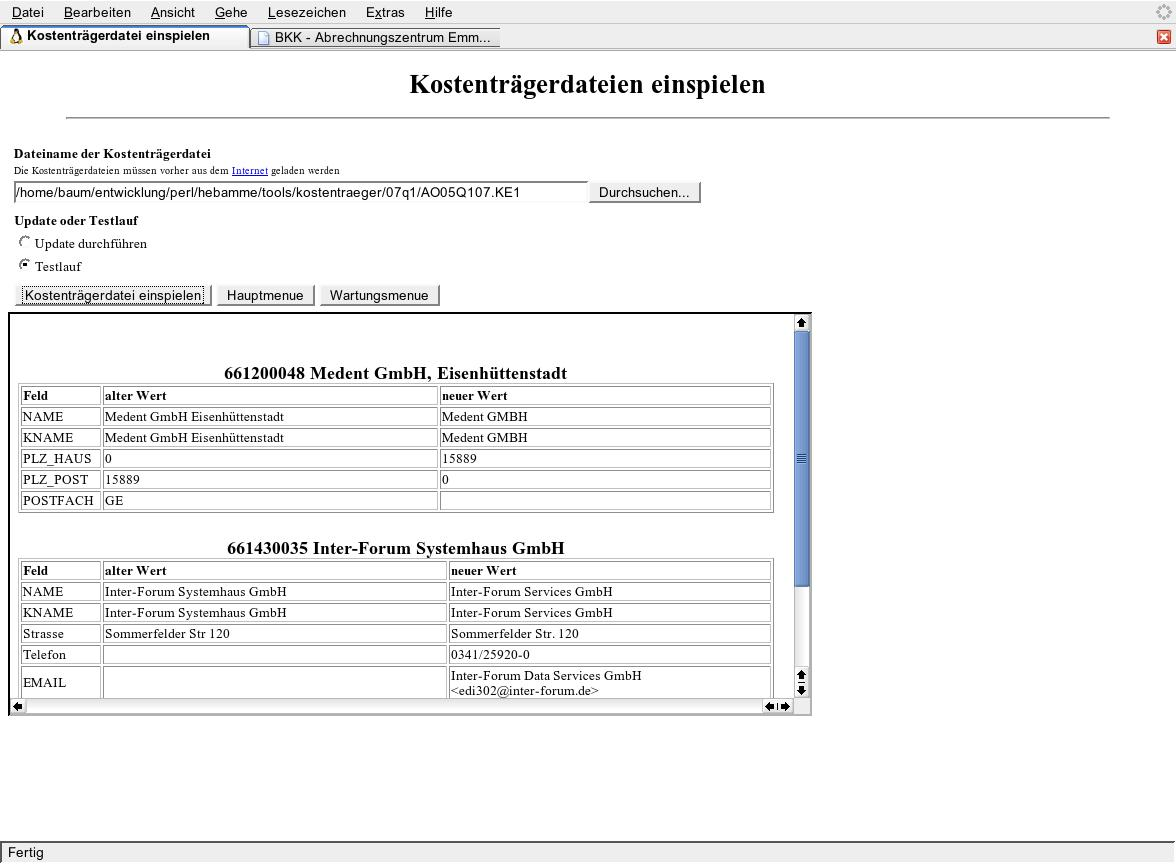
\includegraphics[width=9cm]{kostentraegerdateien}
\caption{Kostenträgerdateien einspielen\label{kostentraegerdateien:fig}}
\end{figure}


\paragraph{Beschreibung des Kommandozeilentools}
\index{kostentraeger.pl}
Mit dem Programm \verb|kostentraeger.pl| im Verzeichnis \verb|tools| können
die Kostenträgerdateien der Krankenkassen
automatisch eingelesen werden. Das Programm muss wie folgt aufgerufen werden:\\
\\
\verb|kostentraeger.pl Optionen|. \\
\\
Folgende Optionen sind möglich:
\begin{compactdesc}
\item\textbf{-h} (Help) gibt eine Bedienungshilfe aus.
\item\textbf{-p} (Pfad) Pfad zu den Kostenträgerdateien.
\item\textbf{-f} (File) die Kostenträgerdatei.
\item\textbf{-o} (Out) der Inhalt der Kostenträgerdatei werden durch TAB \verb|\t| getrennt
ausgegeben. Dadurch ist es möglich Ausgabe in einer Datei zu speichern und
z.B. in einer Tabellenkalkulation weiter zu verarbeiten oder es kann
ein Ladebestand für eine Datenbank generiert werden.
\item\textbf{-c} (Check) Vergleich der Krankenkassen aus der Datenbank mit den Daten aus
der Eingabedatei. Krankenkassen die nicht im Datenbankbestand vorhanden sind,
werden als neue Krankenkassen ausgegeben.
\item\textbf{-n} (New) Ausgabe der Krankenkassen, deren Daten sich zwischen der Eingabedatei
und dem Datenbankbestand unterscheiden, inkl. der Felder, die sich geändert
haben. Nur sinnvoll in Kombination mit Option -c.
\item\textbf{-u} (Update) Geänderte Daten aus der Eingabedatei überschreiben Werte in
der Datenbank. Nur sinnvoll in Kombination mit Option -c.
\item\textbf{-d} (Delete) Es werden die Krankenkassen ausgegeben, die sich in der
Datenbank, aber nicht in der Eingabedatei befinden.
\item\textbf{-v} (Verbose) jede Menge zusätzliche Ausgabem, ist für Debugging sinnvoll.
\end{compactdesc}

\paragraph{Beispiele}
\begin{compactdesc}
\item\textbf{kostentraeger.pl -p kostentraeger/06q2/ -f IK05Q206.KE1 -o}\\
Ausgabe aller Krankenkassen aus der Kostenträgerdatei IK05Q206.KE1 aus 
dem Verzeichnis kostentraeger/06q2/.
\item\textbf{kostentraeger.pl -p kostentraeger/06q2/ -f IK05Q206.KE1 -c}\\
Ausgabe der neuen Krankenkassen aus der Datei IK05Q206.KE1 und Ausgabe, bei 
wie vielen Krankenkassen sich Änderungen, bzw. sich keine Änderungen 
ergeben haben.
\item\textbf{ kostentraeger.pl -p kostentraeger/06q2/ -f IK05Q206.KE1 -c -n}\\
Ausgabe der neuen Krankenkassen und Ausgabe aller geänderten Kassen, inkl.
der Angabe, welche Felder sich geändert haben.
\item\textbf{ kostentraeger.pl -p kostentraeger/06q2/ -f IK05Q206.KE1 -c -n -u}\\
Ausgabe der neuen Krankenkassen und Ausgabe aller geänderten Kassen, inkl.
der Angabe, welche Felder sich geändert haben und update auf die
Datenbank durchführen.
\end{compactdesc}


\subsection{Verarbeitung der öffentlichen Schlüssel der
Datenannahmestellen\label{anhang:pubkey}}
\index{\"offentliche Schlüssel}
\index{Public Keys}
Damit der elektronische Datenaustausch mit den Krankenkassen durchgeführt
werden kann, ist es notwendig die Rechnungsdaten zu verschlüsseln.
Das in \tinyHeb\/ genutzte Verschlüsselungsverfahren ist PKCS\#7\footnote{Wer sich für Details der Verschlüsselungsalgorithmen interessiert, kann diese z.B. in \cite{buchmann} nachlesen. Mathe Leistungskurs oder besser einige Semester Mathematik Studium sind Voraussetzung für die Lektüre.}.
Wesentlicher Bestandteil der Verschlüsselung ist der so genannte public
key der Datenannahmestelle.

Die öffentlichen Schlüssel der Datenannahmestellen stehen im Internet
unter der Adresse 
{\href{ftp://trust.itsg.de/dale/}{\nolinkurl{ftp://trust.itsg.de/dale/}}}
zum Download zur Verfügung. Zwei Dateien sind an dieser Stelle von Interesse:
\begin{enumerate}
\item
\index{gesamt-pkcs.key}
\verb|gesamt-pkcs.key| enthält alle öffentlichen PKCS\#7 Schlüssel, unabhängig,
ob es sich um eine Datenannahmestelle oder eine Hebamme handelt.
\item
\index{annahme-pkcs.key}
\verb|annahme-pkcs.key| enthält die öffentlichen PKCS\#7 Schlüssel der
Datenannahmestellen.
\end{enumerate}
\index{key.pl}
Die Schlüssel aus den Dateien können entweder aus der Kommandozeile 
mit dem Programm  \verb|key.pl| aus dem Verzeichnis \verb|tools| in den
Datenhaushalt von \tinyHeb\/ eingelesen werden, oder über die Maske
``öffentliche Schlüssel der Datenannahmestellen einspielen'', die aus
dem Wartungsmenue aufgerufen werden kann.


\paragraph{Maske öffentliche Schlüssel der Datenannahmestellen
einspielen}
\index{Datenannahmestelle!\"offentlicher Schlüssel}
Die Maske ``öffentliche Schlüssel einspielen'' ist in zwei Bereiche
geteilt. Im oberen Teil der Maske lässt sich einstellen, welche 
Schlüsseldatei eingespielt und ob ein Testlauf oder Update durchgeführt
werden soll.

Der Dateiname der Schlüsseldatei muss im Feld
\feld{Dateiname der Schlüsseldatei} angegeben werden. Über den Knopf
\knopf{Durchsuchen} kann alternativ ein Dateibrowser geöffnet werden,
über den die Datei ausgewählt werden kann.

Bevor ein Update auf die Datenbank gemacht wird, ist es sinnvoll einen
Testlauf durchzuführen, um zu prüfen, welche Daten in der Datei enthalten
sind. Dazu ist \feld{Testlauf} zu markieren. 

Über den Knopf \knopf{Schlüsseldatei einspielen} kann der Testlauf,
resp. das Update auf die Datenbank gestartet werden. Die Verarbeitung
kann je nach Rechneraustattung und welche Datei man gewählt hat, einige
Zeit in Anspruch nehmen. Es sollte solange gewartet werden, bis
im unteren Bereich der Maske keine Ausgabe mehr erfolgt.

Im unteren Bereich der Maske wird angezeigt, welche Informationen in
der eingelesenen Schlüsseldatei vorhanden ist. Als Überschrift wird
bei jedem Zertifikat die IK-Nummer und die Kurzbezeichnung zu dieser
IK-Nummer angezeigt\footnote{natürlich nur dann, wenn diese Information
im Datenhaushalt vorhanden ist.}. Folgende Informationen werden
zusätzlich ausgegeben.

\begin{description}
\item[Seriennummer]
Jedes Zertifikat besitzt eine eindeutige Seriennummer. Diese wird hier
angezeigt.

\item[Organisation]
Organisationsbezeichnung für die das Zertifikat ausgestellt wurde.

\item[Ansprechpartner]
Ansprechpartner für das Zertifikat und ``Inhaber'' des privaten Schlüssels
zu diesem Zertifikat.

\item[Gültig von]
Ab wann kann dieses Zertifikat genutzt werden.

\item[Gültig bis]
Bis wann ist dieses Zertifikat gültig.

\item[Herausgeber]
Wer ist Zertifizierungsstelle für dieses Zertifikat.

\item[Länge des Schlüssels]
Wie lang ist der Schlüssel dieses Zertifikates. Ist die Länge des Schlüssels
kleiner als 2000 Bit, wird die Verarbeitung abgebrochen. Vermutlich wurde
versucht die PEM Version der Schlüsseldatei einzulesen. Bei der PEM Version
wird mit Schlüssellängen von 768 Bit gearbeitet.

\item[Algorithmus des Schlüssels]
Mit welchem Verfahren wurde der Schlüssel erzeugt. Hier sollte b.a.w. immer
rsaEncryption stehen.

\item[Status Datenaustausch]
Hier wird angezeigt, ob es sich bei dem Schlüssel dieser Organisation
um eine Datenannahmestelle
handelt oder nicht. Falls es sich um eine Datenannahmestelle handelt, wird
der Schlüssel eingelesen und der Status des Datenaustausches, wie er in
\tinyHeb\/ parametrisiert ist, angezeigt.

\end{description}

\begin{figure}[H]
\centering
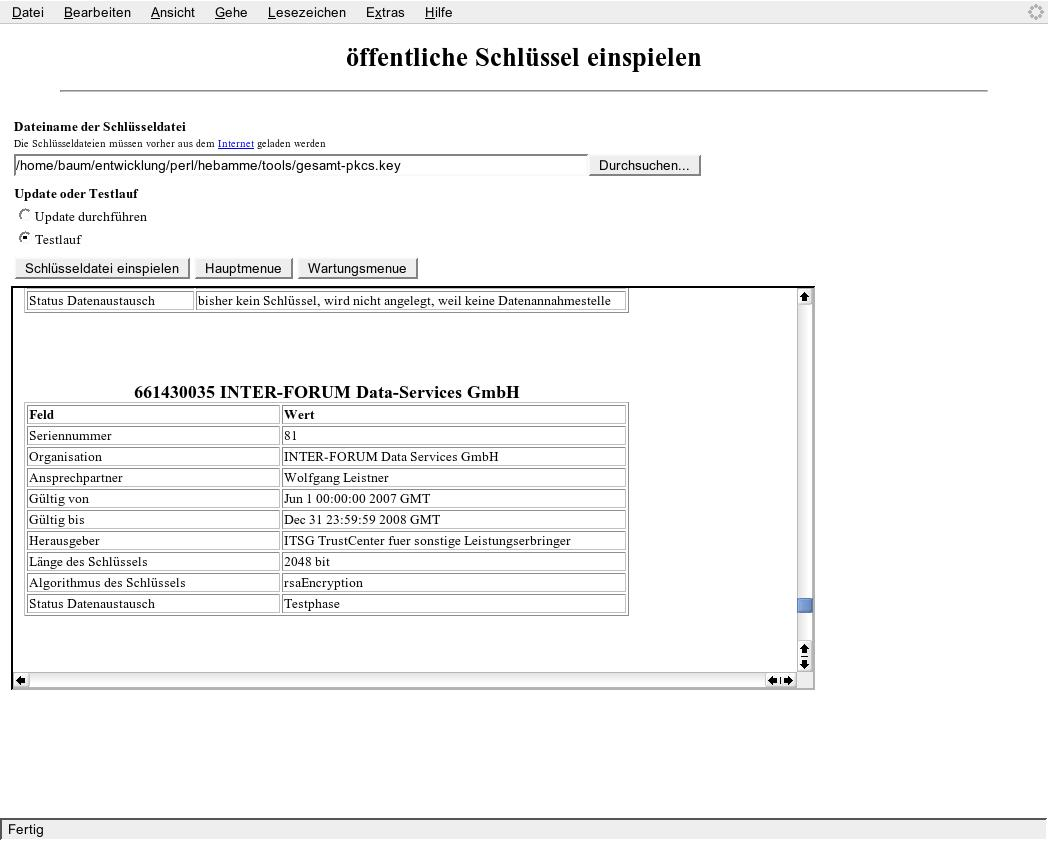
\includegraphics[width=9cm]{schluesseldateien}
\caption{Schlüsseldateien einspielen\label{schluesseldateien:fig}}
\end{figure}


\paragraph{Beschreibung des Kommandozeilen Tools}
Mit dem Programm \verb|key.pl| im Verzeichnis \verb|tools| können die
Schlüsseldateien der Datenannahmestellen automatisch eingelesen werden.
Das Programm muss wie folgt aufgerufen werden:\\
\\
\verb|key.pl| Optionen.\\
\\
Folgende Optionen sind möglich:
\begin{compactdesc}
\item
\textbf{-h} (Help) gibt eine Bedienungshilfe aus.
\item
\textbf{-p} (Pfad) Pfad zu der Schlüsseldatei, kann auch entfallen, wenn sich
die Schlüsseldatei im Verzeichnis \verb|tools| befindet.
\item
\textbf{-f} (File) Name der Schlüsseldatei.
\item
\textbf{-s} (Save) speichert die einzelnen Zertifikate in jeweils 
eigener Datei.
Die generierten Dateinamen lauten IK-Nummer.pem. So kann man zum Beispiel sein
eigenes Zertifikat aus der Datei \verb|gesamt-pkcs.key| extrahieren.
\item
\textbf{-o} (Out) In welches Verzeichnis sollen die einzelnen öffentlichen
Schlüssel der Datenannahmestellen geschrieben werden. Wird dieser Parameter
nicht gesetzt, wird automatisch das Verzeichnis \verb|keys| genutzt. Das
Verzeichnis zum Schreiben der einzelnen Schlüssel muss vorhanden sein.
\item
\textbf{-u} (Update) vorhandene Daten aus der Eingabedatei überschreiben Werte
 in der Datenbank.
\item
\textbf{-v} (Verbose) jede Menge zusätzliche Ausgabem, ist für Debugging 
sinnvoll oder wenn man überprüfen möchte, ob neue Schlüssel dazu gekommen
sind.
\item
\textbf{-c} kopiert das Zertifikat der Hebamme an die richtige Stelle für
die weitere Verarbeitung. Siehe auch Seite \pageref{anhang:eigenes_cert}.
\item
\textbf{-t} (hTml) es wird HTML formatierte Ausgabe generiert.
\end{compactdesc}


\paragraph{Beispiele}
\begin{compactdesc}
\item
\textbf{key.pl -s -f annahme-pkcs.key}\\
Gibt Informationen zu den in der Datei \verb|annahme-pkcs.key| enthaltenen
Schlüsseln aus. Alle einzelnen Schlüssel werden im Verzeichnis keys mit
dem Dateinahmen ik-nummer.pem gespeichert.
\item
\textbf{key.pl -v -s -f gesamt-pkcs.key}\\
Gibt Informationen zu den in der Datei \verb|gesamt-pkcs.key| enthaltenen
Schlüsseln aus. Zusätzlich wird der Gültigkeitszeitraum des Zertifikates
ausgegeben. Alle einzelnen Schlüssel werden im Verzeichnis keys mit
dem Dateinahmen ik-nummer.pem gespeichert.
Diesen Befehl solltet Ihr mal ausprobieren und die Ausgabe nach Hebamme
durchsuchen, dann bekommt Ihr einen Eindruck wie viele Hebammen über ein
PKCS\#7 Zertifikat verfügen.
\item
\textbf{key.pl -s -f annahme-pkcs.key -o annahme}\\
Gibt Informationen zu den in der Datei \verb|annahme-pkcs.key| enthaltenen
Schlüsseln aus. Alle einzelnen Schlüssel werden im Verzeichnis \verb|annahme|
 mit dem Dateinahmen ik-nummer.pem gespeichert.
\item
\textbf{key.pl -s -f annahme-pkcs.key -o annahme -u}\\
Gibt Informationen zu den in der Datei \verb|annahme-pkcs.key| enthaltenen
Schlüsseln aus. Alle einzelnen Schlüssel werden im Verzeichnis \verb|annahme|
 mit dem Dateinahmen ik-nummer.pem gespeichert. Zusätzlich werden die
Schlüssel in den \tinyHeb\/ Datenhaushalt übernommen. 
\end{compactdesc}


\section{zusätzliche Provider im elektronischen Datenaustausch\label{anhang:provider}}
Im Rahmen des elektronischen Datenaustausches ist es ggf. notwendig
unterschiedliche E-Mail Provider für den Datenaustausch zu nutzen, insb.
weil das ARZ-Emmendingen in der Regel keine E-Mails vom Provider Arcor
akzeptiert.
Es gibt zwei Möglichkeiten die notwendigen Informationen zu hinterlegen.
Entweder durch Editieren der Datei \verb|.xauftragrc| oder
seit \tinyHeb\/ Version 1.1.0 aus der Anwendung \verb|xauftrag.pl|.

\paragraph{Aus der Anwendung xauftrag.pl}

\begin{figure}[ht]
\centering
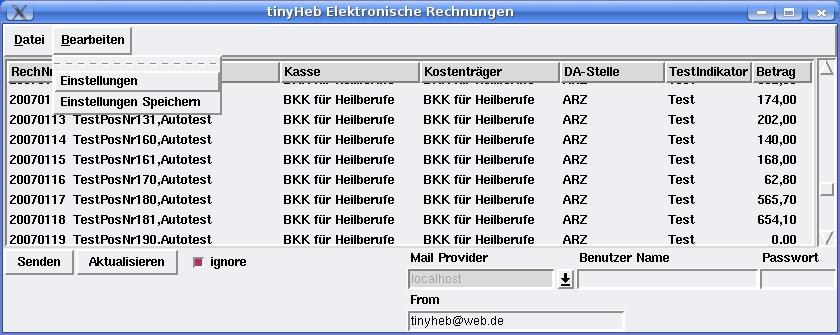
\includegraphics[width=80mm]{xauftrag_bearbeiten}
\caption{Elektronische Rechnungen, Maileinstellungen \label{anhang:xauftrag:fig}}
\end{figure}

Dazu ist zunächst die Anwendung \verb|xauftrag.pl| aus dem Verzeichnis
\verb|edifact| zu starten -- siehe dazu auch Kapitel \vref{elekrechnung:kap} 
und Abbildung \vref{anhang:xauftrag:fig}.


Durch Klicken auf Bearbeiten und Einstellungen öffnet sich ein neues 
Fenster (Abbildung \vref{anhang:xauftrag_einstellungen:fig}), 
in dem  Angaben bzgl. der 
einzelnen Provider, bzw. der einzelnen Mail Accounts geändert werden können.

Hat man die Angaben geändert muss der Knopf 
\knopf{Einstellungen übernehmen und Schließen} gedrückt werden, damit die
Änderungen in die laufende Anwendung übernommen werden. Das Fenster schließt
sich nachdem der Knopf gedrückt wurde.
So kann man z.B. zunächst Testen, ob die Änderungen den gewünschten Effekt 
haben. Sollen die Angaben permanent verfügbar sein, muss der Knopf
\knopf{Einstellungen Speichern} aus Abbildung \vref {anhang:xauftrag:fig}
gedrückt werden.

\begin{figure}[ht]
\centering
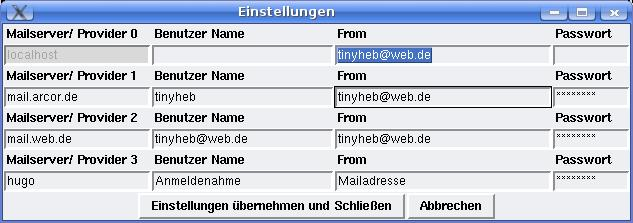
\includegraphics[width=80mm]{xauftrag_einstellungen}
\caption{Elektronische Rechnungen, Maileinstellungen \label{anhang:xauftrag_einstellungen:fig}}
\end{figure}


\paragraph{Durch Editieren der Datei}

Dazu ist es notwendig im Verzeichnis \$HOME/.tinyheb\footnote{wie mir einige WinXP Nutzer geschrieben haben, landet die Datei unter Windows im Verzeichnis \textbackslash tinyheb} die Datei
\verb|.xauftragrc| anzupassen\footnote{unter Vista kann die Datei nur mit
notepad aus der Eingabeaufforderung bearbeitet werden, die ist zu beachten}. 
Diese Datei wird beim ersten Start von 
\verb|xauftrag.pl| mit einigen Beispiel Einträgen automatisch angegelegt.
Diese Einträge sind auf die eigenen Bedürfnisse anzupassen.
Durch TAB \verb|\t| getrennt sind folgende Einträge vorzunehmen:
\begin{enumerate}
\item
Mailserver des Providers, z.B. mail.web.de
\item
Name den man zur Anmeldung beim Provider benötigt, z.B. 
\nolinkurl{tinyheb@web.de}
\item
E-Mail Adresse die bei o.g. Provider genutzt werden soll, z.B.
\nolinkurl{tinyheb@web.de}
\item
Passwort, falls für die Anmeldung beim Provider ein Passwort benötigt wird.
\end{enumerate}
So lassen sich beliebig viele Mail Adressen zum Verschicken von elektronischen
Rechnungen hinterlegen.

\paragraph{Beispiel für die Datei .xauftragrc}
\begin{verbatim}
mail.arcor.de   tiny.heb        tiny.heb@arcor.de       passwort
mail.web.de     anmeldename     mailadresse@provider.de passwort
mail.arcor.de   anmeldename     mail@provider.de        passwort
mail.web.de     tiny.heb@web.de tiny.heb@web.de         passwort
\end{verbatim}


\section{Ein eigenes Zertifikat\label{anhang:eigenes_cert}}
\index{Zertifikat}
In diesem Kapitel ist beschrieben, wie man zu einem eigenen Zertifikat
kommt. Ein solches Zertifikat ist notwendig, wenn man seine Rechnungen
signieren möchte, d.h. mit einer elektronischen Unterschrift versehen
möchte oder muss. Datenannahmestellen wie z.B. Inter-Forum oder Medent
akzeptieren ausschließlich signierte Rechnungen; werden die Rechnungen
nur verschlüsselt, kommt es zu einer Fehlermeldung.

Bevor man an dieser Stelle in der Anleitung weiter liesst, sollte man sich 
das FAQ der ITSG durchlesen. Das findet sich im Internet bei der ITSG:

{\href{http://www.itsg.de/(S(vi2qcf555ulqr4yvshldrt55))/tc_faq.ITSG}{\nolinkurl{http://www.itsg.de/(S(vi2qcf555ulqr4yvshldrt55))/tc_faq.ITSG}}}

Die Generierung und die Übernahme des Zertifikates in \tinyHeb\/ erfolgt
dann in drei Schritten:

\begin{enumerate}
\item
Zunächst muss ein privater Schlüssel und aus diesem eine
\index{privater Schlüssel}
Zertifikatsanfrage generiert werden. Dazu existiert in \tinyHeb\/ das
Programm \verb|genreq.pl| im Verzeichnis \verb|tools|. Nach der Generierung
der Zertifikatsanfrage muss diese an die ITSG per E-Mail geschickt werden,
auch dies erledigt das Programm.
\item
Im nächsten Schritt ist es notwendig, die begleitenden Unterlagen per
Fax oder Papierpost an die ITSG zu schicken.
\item
Sind alle Unterlagen vollständig, generiert die ITSG das eigentliche
Zertifikat, welches man per E-Mail zugeschickt bekommt. Leider habe ich
noch keinen kennengelernt -- aber ich kenne auch nicht viele -- die die
Dateianhänge der ITSG ohne Probleme aus der Mail lösen konnten. Daher
gibt es eine Option im Programm key.pl mit der aus der Datei
gesamt-pkcs.key das eigene Zertifikat ausgelesen werden kann.
\end{enumerate}

\subsection{Zertifikatsanfrage generieren}
Um die Zertifikatsanfrage zu generieren starten man das Programm 
\verb|genreq.pl| aus dem Verzeichnis \verb|tools|. Es öffnet sich
ein Fenster (siehe Abbildung \vref{zertifikat:fig}), 
in dem verschiedene Angaben zu machen sind.

\begin{figure}[H]
\centering
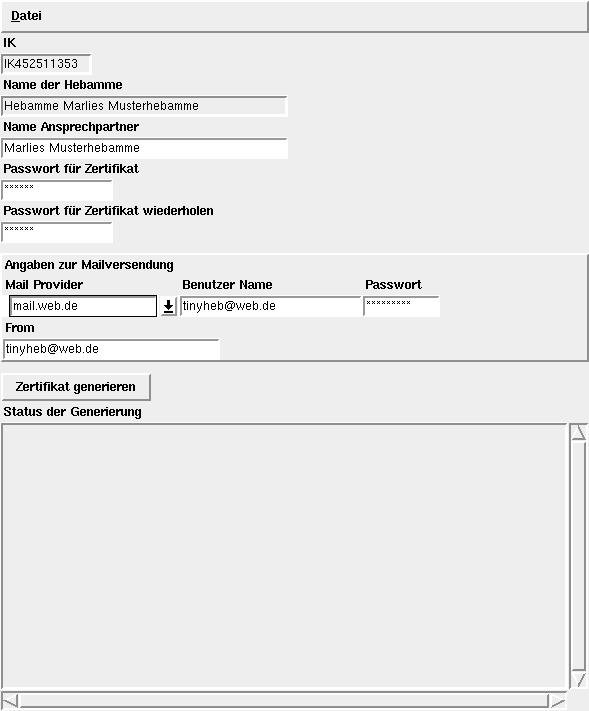
\includegraphics[width=9cm]{certreq}
\caption{\tinyHeb\/ Zertifikatgenerierung\label{zertifikat:fig}}
\end{figure}

\begin{description}
\item[IK]
In dieses Feld wird die IK Nummer der Hebamme aus der \tinyHeb\/ 
Datenbank geschrieben. Das Feld lässt sich nicht ändern. Wer es ändern
möchte, muss dies über die Maske ``Angaben zur Hebamme'' machen.
\item[Name der Hebamme]
In dieses Feld wird der Name der Hebamme, wie er in der \tinyHeb\/
Datenbank hinterlegt ist geschrieben. Das Feld lässt sich nicht ändern. 
Wer es ändern möchte, muss dies über die Maske ``Angaben zur Hebamme'' machen.
Die Bezeichnung Hebamme wird automatisch voran gestellt. Dies lässt sich
nicht ändern.
\item[Name Ansprechpartner]
Hier muss ein Ansprechpartner hinterlegt werden. Im Zweifel ist dies die
Hebamme selbst.
\item[Passwort für Zertifikat]
Hier ist nicht das Passwort des Zertifikates hinterlegt, sondern
das Passwort zu dem entsprechenden privaten Schlüssel. Dieses Passwort
muss man sich sehr gut merken. Es wird später zum Signieren der Rechnungen
benötigt.
\index{Signatur}
\marginline{\Huge\bfseries!}%
\item[Passwort für Zertifikat wiederholen]
Identisch zum Feld \feld{Passwort für Zertifikat}
\item[Angaben zur Mailversendung]
Hier sind die identischen Angaben zu machen, wie bei der elektronischen
Versendung von Rechnungen. Sobald ein Mail Provider ausgewählt wird, 
werden die Felder \feld{Benutzer Name, Passwort} und \feld{From} gefüllt. 
Woher diese
Informationen kommen und wie zusätzliche Provider hinterlegt werden
können ist in Kapitel \vref{anhang:provider} beschrieben.
\end{description}

Durch Klicken des Knopfes \knopf{Zertifikat generieren} wird die Generierung
mit den oben gemachten Angaben gestartet.

Während der Generierung der Zertifikatsanfrage werden einige Fragen gestellt:
\begin{description}
\item[Es existiert schon eine Zertifikatsanfrage, soll diese überschrieben
werden?]
Falls man schon ein Zertifikat besitzt, dieses aber abgelaufen ist, sollte
man die Frage mit 'Ja' beantworten. Hat man schon eine Zertifikatsanfrage
generiert, diese aber nicht an die ITSG per Mail geschickt, kann man diese
Frage mit 'ja' beantworten. 

In allen anderen Fällen sollte man genau
überlegen was man tut und ggf. in der \tinyHeb\/ Mailingliste nachfragen.

\item[Es existiert schon ein privater Schlüssel, soll ein neuer generiert
werden?]
Falls man schon über einen privaten Schlüssel verfügt und keinen neuen
generieren möchte, muss man diese Frage mit 'Nein' beantworten. In diesem
Fall ist zu beachten, das im Feld \feld{Passwort für Zertifikat} des
Passwort des existierenden Schlüssels angegeben wird. 

Falls ein neuer
Schlüssel generiert werden soll, kann oder sollte ein neues Passwort vergeben
werden.

\item[Soll eine verschlüsselte Sicherung des Passwortes angelegt werden?]
Wer sich sicher ist, dass er niemals das Passwort seines privaten Schlüssels
vergisst, kann diese Frage mit 'nein' beantworten. Falls man das Passwort
trotzdem vergisst, muss ein neues Zertifikat beantragt werden.

Wenn die Frage mit 'ja' beantwortet wird, wird eine eine verschlüsselte
Kopie des Passwortes angelegt. Diese Kopie kann nur vom Author von 
\tinyHeb\/ entschlüsselt werden und dies nur dann, wenn diesem die Kopie 
zugeschickt wird. Es ist zu hoffen, dass nie ein Nutzer diese ``Service''
in Anspruch nehmen muss.

\end{description}

Im Rahmen der Generierung werden verschiedene Statusmeldungen erstellt.
Wichtig ist die MD5 Signatur, die auch Prüfsumme, Komprimat des Schlüssels
\marginline{\Huge\bfseries!}%
oder Fingerprint genannt wird. Diese Ziffernfolge ist unterschrieben an
die ITSG zu schicken. Im konkreten Fall wäre dies:
\index{Prüfsumme}
\verb|fd:7a:0f:07:e5:90:0f:er:a5:f2:35:53:25:e6:02:2b|.

\begin{description}
\item[Soll das Zertifikat per E-Mail an die ITSG geschickt werden?]
Diese Frage sollte mit 'Ja' beantwortet werden.

\item[Soll ich die Dateien in die korrekten Verzeichnisse kopieren?\\
 Alte Zertifikate werden überschrieben]
Auch diese Frage sollte mit 'Ja' beantwortet werden. Eine Ausnahme ist nur
gegeben, wenn man schon über ein Zertifikat verfügt und dieses noch nicht 
abgelaufen ist. Dieser Sachverhalt sollte eigentlich nicht vorkommen, da man
sein Folgezertifikat erst dann bestellen sollte, wenn das alte Zertifikat
ungültig geworden ist.
\end{description}


An dieser Stelle sollte eine Sicherung des Verzeichnisses 
\verb|$HOME/.tinyheb/|\footnote{unter Windows im Verzeichnis \textbackslash tinyheb}
durchgeführt und an einem \textbf{sehr} sicheren Ort
verwahrt werden, falls z.B. nach einem Systemabsturz der private
Schlüssel wieder für \tinyHeb\/ nutzbar gemacht werden soll.
\marginline{\Huge\bfseries!}%

Damit ist Schritt eins erledigt.

\begin{figure}[H]
\centering
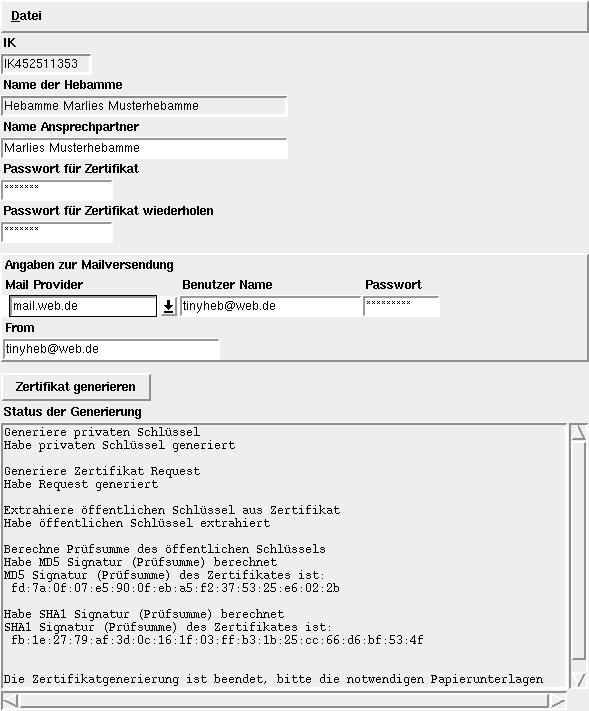
\includegraphics[width=9cm]{certreq2}
\caption{\tinyHeb\/ Zertifikatgenerierung\label{zertifikat2:fig}}
\end{figure}

\subsection{begleitende Unterlagen}
Neben den Unterlagen, die im FAQ der ITSG beschrieben sind, hilft ein
kleines Anschreiben. Es reicht folgendes:
\begin{verbatim}
Hebamme
Marlies Musterhebamme
Strasse
Ort
Tel. 
IK 123456789



Atos Origin GmbH
ITSG Trustcenter
Postach 1225
49702 Meppen

                                                     Ort, den tt.mm.jjjj

Unterlagen zur Zertifikatsanfrage 123456789


Sehr geehrte Damen und Herren,

hier wie von Ihnen gewünscht der unterschriebene Ausdruck des 
öffentlichen Schlüssels / Komprimats:

Komprimat zum Schlüssel (MD5 Hash)
fd:7a:0f:07:e5:90:0f:er:a5:f2:35:53:25:e6:02:2b


Mit freundlichen Grüßen

Marlies Musterhebamme
\end{verbatim}

Das ist alles, was man in Schritt zwei machen muss.

\subsection{Das Zertifikat in \tinyHeb\/ übernehmen}
Sind alle Unterlagen vollständig bei der ITSG eingetroffen, dauert es ein
bis zwei Tage, bis das eigentliche Zertifikat generiert ist. Über diesen
Sachverhalt bekommt man eine Mail, die folgende Betreff Zeile hat:
\verb|12345678.p7c|, d.h., die IK-Nummer der Hebamme ohne Prüfziffer.

Der Dateianhang dieser Mail enthält das eigentliche Zertifikat. Leider 
ist der Anhang \verb|uucoded|, daher habe ich es nicht geschafft, mit
normalen Bordmitteln den Anhang zu lösen. Es gibt in \tinyHeb\/
eine andere Möglichkeit das Zertifikat an der korrekten Stelle abzulegen.

Man lädt sich die Datei \verb|gesamt-pkcs.key| vom FTP Server der ITSG
herunter
\index{gesamt-pkcs.key}
{\href{ftp://trust.itsg.de/dale/}{\nolinkurl{ftp://trust.itsg.de/dale/}}}
und benutzt diese als Eingabe für das Programm \verb|key.pl| 
(siehe auch Anhang \vref{anhang:pubkey}) oder 
\verb|xkey.pl| (seit \tinyHeb\/ Version 1.2.0) aus dem
Verzeichnis \verb|tools|. 

Es ist zu beachten, dass die Datei
\index{gesamt-pkcs.key}
\verb|gesamt-pkcs.key| täglich von der ITSG neu generiert wird, d.h.,
dass eigene Zertifikat ist erst einen Tag nach der Bestätigungsmail in
der Datei enthalten.

\paragraph{Aufruf xkey.pl}
\index{xkey.pl}
\index{eigenes Zertifikat einlesen}
\verb|xkey.pl| kann unter Windows per Doppelklick und unter Linux ganz
normal gestartet werden. Es öffnet sich ein neues Fenster (siehe 
Abbildung \vref{xkey:fig}), in dem verschiedene Angaben zu machen sind.

\begin{figure}[H]
\centering
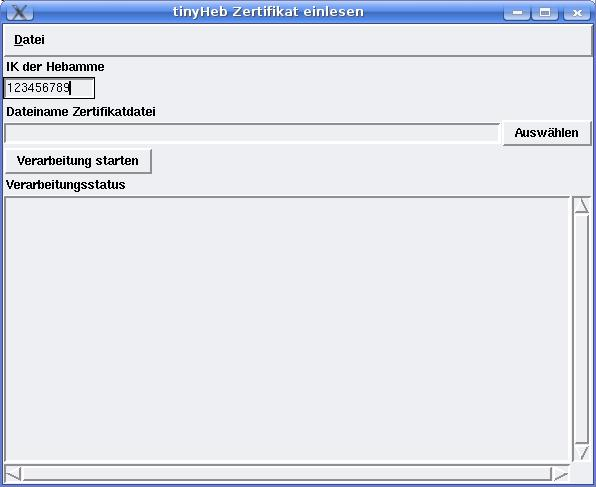
\includegraphics[width=9cm]{xkey}
\caption{\tinyHeb\/ Einlesen des eigenen Zertifikates mit xkey.pl\label{xkey:fig}}
\end{figure}

\begin{description}
\item[IK der Hebamme]
Hier ist die IK Nummer der Hebamme anzugeben, deren Zertifikat übernommen
werden soll. Dieses Feld wird automatisch mit dem Wert aus den Parametern
vorbelegt.
\item[Dateiname der Zertifikatdatei]
Hier ist der Name der Zertifikatdatei anzugeben, in der Regel 
\verb|gesamt-pcks.key|. Über den Knopf \knopf{Auswählen} öffnet sich ein
Dialogfenster, über das der Dateinahme ausgewählt werden kann.
\end{description}

Sind diese beiden Angaben gemacht, kann über den Knopf 
\knopf{Verarbeitung starten} das Einlesen des eigenen Zertifikates
gestartet werden.
Falls das Zertifikat der Hebamme in der Datei enthalten ist, wird es
in das \$HOME Verzeichnis\footnote{unter Windows im Verzeichnis \textbackslash tinyheb\textbackslash privkey} des angemeldeten Benutzers kopiert.
Im Rahmenn Verarbeitungsstatus wird dies angezeigt.
\begin{verbatim}
Habe Zertifikat fuer 123456789 nach /home/xx/.tinyheb/privkey/123456789.pem 
kopiert.
\end{verbatim}
Das Einlesen kann in Abhängigkeit der Rechnerausstattung einige Zeit 
in Anspruch nehmen, da ca. 8000 Zertifikate verarbeitet werden müssen
\footnote{unter Linux kann die Verarbeitung erheblich beschleunigt werden,
indem man das Modul Crypt::OpenSSL::X509 installiert}

\paragraph{Aufruf key.pl}
\verb|key.pl| muss dann mit folgenden Parametern aufgerufen werden:
\\
\verb|key.pl -c -f gesamt-pkcs.key|\footnote{Der Aufruf funktioniert
natürlich nur dann, wenn man vorher die Datei gesamt-pkcs.key im
Verzeichnis tools gespeichert hat}\\
\\
Falls das Zertifikat der Hebamme in der Datei enthalten ist, wird es
in das \$HOME Verzeichnis\footnote{unter Windows im Verzeichnis \textbackslash tinyheb\textbackslash privkey} des angemeldeten Benutzers kopiert.
\begin{verbatim}
Habe Zertifikat fuer 123456789 nach /home/xx/.tinyheb/privkey/123456789.pem 
kopiert.
\end{verbatim}

Damit ist das Zertifikat in \tinyHeb\/ verfügbar und die Rechnungen können
mit einer Signatur versehen werden. Damit dies auch wirklich passiert,
muss der Parameter Signatur der einzelnen Datenannahmestellen auf 
PKCS\#7 Signatur gestellt werden 
(siehe Kapitel \vref{datenannahmestellen:abs}). 
Zukünftig wird \tinyHeb\/ nach dem
Passwort fragen, wenn die Rechnungen verschickt werden.

An dieser Stelle sollte unbedingt eine Sicherung des Verzeichnisses 
\verb|$HOME/.tinyheb/privkey/|\footnote{unter Windows im Verzeichnis \textbackslash tinyheb\textbackslash privkey}
durchgeführt und an einem \textbf{sehr} sicheren Ort
verwahrt werden, falls z.B. nach einem Systemabsturz der private
Schlüssel wieder für \tinyHeb\/ nutzbar gemacht werden soll.
\marginline{\Huge\bfseries!}%



\chapter{Hintergrundinformationen}

In diesem Kapitel sind einige Hintergrundinformationen aufbereitet, die
die Fehlersuche oder auch das Verständnis für die Abläufe in \tinyHeb\/
erleichtern.

\section{Generierung von elektronischen Rechnungen}

In diesem Abschnitt wird beschrieben, wie eine elektronische Rechnung
generiert wird, auf welche Daten zugegriffen wird und welche
Zwischendateien generiert werden.

\paragraph{Voraussetzungen}
Um eine elektronische Rechnung generieren zu können, ist es für \tinyHeb\/
notwendig, dass eine Papierrechnung existiert, d.h. die einzelnen
Rechnungspostionen sind mit dem Status 20 und einer Rechnungsnummer
versehen.

Mit dem Programm \verb|xauftrag.pl| werden genau diese Rechnungen zur 
Anzeige gebracht. Dabei ist folgende Einschränkung zu beachten, existiert
zu einer Krankenkasse keine oder keine parametrisierte Datenannahmestelle
wird die Rechnung nicht angezeigt. Existiert kein öffentlicher Schlüssel
\index{Datenannahmestelle!\"offentlicher Schlüssel} zu der Datenannahmestelle wird die Rechnung
nicht angezeigt.

\subsection{Generierung der elektronischen Rechnung}
Die Generierung der elektronischen Rechnung erfolgt in zwei Phasen.
In der ersten Phase wird überprüft, ob eine elektronsche Rechnung
fehlerfrei produziert werden kann.
In der zweiten Phase wird die echte elektronische Rechnung erzeugt.

\paragraph{Phase eins}
In der ersten Phase wird u.a. geprüft, ob folgende Angaben ermittelt werden
können:

\begin{description}
\item[Angaben zur Frau]
Alle notwendigen Daten zur Frau für die eine Rechnung erstellt werden soll,
werden erst jetzt aus der Datenbank gelesen, d.h. es ist möglich
nachträglich Angaben zu ändern, wie z.B. den Versichertenstatus.
\item[Angaben zur Hebamme]
Alle notwendigen Daten zur Hebamme die eine Rechnung erstellt,
werden erst jetzt aus der Datenbank gelesen, d.h. es ist möglich
nachträglich Angaben zu ändern, wie z.B. die E-Mail Adresse.
\item[Angaben zur Krankenkasse]
Alle notwendigen Daten zur Krankenkasse werden erst jetzt aus der Datenbank 
gelesen. Das Lesen der Daten erfolgt auf Basis der IK-Nummer der Krankenkasse,
wie diese zum Zeitpunkt des Speicherns der Papierrechnung in den Stammdaten
der Frau hinterlegt war. D.h. es ist nicht möglich diese IK-Nummer
nachträglich zu ändern.
Abhängige Daten, wie z.B. die IK-Nummer des Kostenträgers oder der
Datenannahmestelle können nachträglich geändert werden\footnote{siehe
dazu Maske Krankenkassendaten}. 
\item[E-Mail Adresse der Datenannahmestelle]
Es wird geprüft, ob eine E-Mail Adresse zur Datenannahmestelle vorhanden ist.
Es wird nicht geprüft, ob die E-Mail Adresse korrekt ist.
\item[Signierung]
Falls die Rechnung signiert werden soll, wird geprüft, ob dies mit den
bisherigen Angaben möglich ist. Dazu zählen der private Schlüssel der
Hebamme, das Passwort zum privaten Schlüssel und  das Zertifikat der Hebamme.
\item[Verschlüsselung]
Falls die Rechnung signiert werden soll, wird geprüft, ob dies mit den
bisherigen Angaben möglich ist. Dazu zählen der öffentliche Schlüssel
der Datenannahmestelle und eine korrekte OpenSSL Installation.
\end{description}

Folgende Zwischendateien werden während der ersten Phase im Verzeichnis
\$HOME/.tinyheb/tmp/\footnote{unter Windows im Verzeichnis \textbackslash tinyheb\textbackslash tmp}
generiert:
\begin{description}
\item[zik.pem]
In dieser Datei wird der öffentliche Schlüssel der Datenannahmestelle
gespeichert. Wer sich diesen Schlüssel in Klartext ansehen möchte, kann
dies mit OpenSSL machen:
\verb|openssl x509 -in zik.pem -text|
\item[test\_enc]
In dieser Datei sind die unverschlüsselten Nutzdaten der Rechnung enthalten.
\item[test\_enc.sig]
In dieser Datei sind die signierten Nutzdaten der Rechnung enthalten. Falls
die Daten nicht signiert wurden, ist diese Datei identisch zur Datei
\verb|test_enc|. Wer sich die signierten Daten im ASN.1 Format ansehen
möchte, kann dies mit OpenSSL machen: 
\verb|openssl asn1parse -in test_enc.sig -inform DER -dump|
\item[test\_enc.enc]
In dieser Datei sind die verschlüsselten Nutzdaten der Rechnung enthalten.
Falls die Daten nicht verschlüsselt wurden, ist diese Datei identisch zur
Datei \verb|test_enc.sig|. Wer sich die signierten Daten im ASN.1 Format
ansehen möchte, kann dies mit OpenSSL machen:\\
\verb|openssl asn1parse -in test_enc.enc -inform DER -dump|
\end{description}

Mit der Generierung der oben beschriebenen Dateien ist Phase eins der
Rechnungsgenerierung abgeschlossen.


\paragraph{Phase zwei}
In Phase zwei werden ähnliche Dateien wie in Phase eins beschrieben erzeugt.
Allerdings werden in Phase zwei die korrekten Datenaustauschreferenzen und
der korrekte Dateiname genutzt.

Der Dateinahme beginnt entweder mit TSOL oder mit ESOL. 

\index{\textbf{TSOL}}
TSOL, falls die Rechnung im Testbetrieb oder der Eprobungsphase 
übermittelt werden soll.

\index{\textbf{ESOL}}
ESOL, falls die Rechnung im Echtbetrieb übermittelt wird.

Danach folgt eine 4-stellige laufende Nummer, bei dieser Nummer handelt es
sich um die Datenaustauschreferenz (siehe \vref{datenannahmestellen:abs}),
so ensteht zum Beispiel der Dateiname \verb|TSOL0009|. Diese Datei enthält die
Nutzdaten der Rechnung. Die Datei \verb|TSOL0009.sig| enthält die signierten
Nutzdaten, \verb|TSOL0009.enc| die verschlüsselten Nutzdaten. Die Datei 
\verb|TSOL0009.AUF| enthält die Auftragsdaten zu dieser Rechnung.

Nachdem diese Dateien im Verzeichnis \$HOME/.tinyheb/tmp/\footnote{unter Windows im Verzeichnis \textbackslash tinyheb\textbackslash tmp}
generiert wurden und die Rechnung erfolgreich über das Internet 
verschickt werden konnte, werden diese Dateien in ein Unterverzeichnis 
unterhalb tmp verschoben. Dieses Verzeichnis trägt der Namen (IK-Nummer)
des physikalischen Empfängers der Datei, z.B. 107436557.




\section{Sicherheit in \tinyHeb\/}

In diesem Abschnitt wird beschrieben, wie sicher, resp. unsicher 
\tinyHeb\/ ist und wie man es mit bestimmten Handgriffen sicherer macht.
Es ist vermutlich notwendig ein gewisses technisches Verständnis für dieses
Kapitel mitzubringen.

Die Ausführungen sind nach bestem Wissen gemacht, ersetzen jedoch in 
keinem Fall die Lektüre der entsprechenden Programmdokumentation zum
eingesetzten Betriebssystem\footnote{WinXP, Linux um Beispiele zu nennen}, 
der MySQL Datenbank und dem Webserver Apache.

\paragraph{Sicherheit im Betriebssystem}
Einige Betriebssysteme haben eine integrierte Firewall, wer diese abschaltet,
öffnet Angreifern natürlich Tür und Tor um auf die entsprechenden Dienste
zuzugreifen.\footnote{zu diesen Diensten gehören auch Apache und MySQL}
D.h. für \tinyHeb\/ wer keine Firewall hat, der könnte ein Problem mit
der Sicherheit seiner Daten bekommen.
Wer eine Firewall hat, der muss für \tinyHeb\/ die Ports 80 für Apache und
3306 für MySQL für den Zugriff von aussen -- aus dem Internet und/oder
ggf. des LANs -- schließen.

Von Interesse für \tinyHeb\/ ist noch die Datei \verb|privkey.pem| in
der der private Schlüssel zum Signieren von Rechnungen enthalten ist.
Diese Datei sollte nur und ausschließlich Leserechte für den Benutzer
haben, der diese benötigt um Rechnungen zu signieren. 
Damit die Datei nicht versehentlich gelöscht wird,
sollte kein Benutzer Schreibrechte für diese Datei besitzen.


\paragraph{Sicherheit des Webservers}
Der Apache ist ein vollständiger Webserver, der für die Nutzung von
\tinyHeb\/ benötigt wird, d.h. es ist keine Verbindung zum Internet
notwendig, um \tinyHeb\/ Nutzen zu können.

Die Konfigurationsdatei des Webservers enthält für \tinyHeb\/ im Standard
folgende Einstellungen:
\begin{verbatim}
Alias /tinyheb/ "/srv/www/cgi-bin/tinyheb/"

<Directory /srv/www/cgi-bin/tinyheb>
        AllowOverride None
        Options -Indexes +ExecCGI +FollowSymLinks
        AddHandler cgi-script pl
        Order allow,deny
        Allow from all
</Directory>
\end{verbatim}

Mit diesen Einstellungen ist ein Zugriff auf \tinyHeb\/ bei bestehender
Internetverbindung jederzeit möglich! Wenn keine Firewall wie oben 
beschrieben genutzt wird.

Mit folgenden Einstellungen wird die Zugriffsmöglichkeit auf den lokalen
Rechner eingeschränkt:
\begin{verbatim}
Alias /tinyheb/ "/srv/www/cgi-bin/tinyheb/"

<Directory /srv/www/cgi-bin/tinyheb>
        AllowOverride None
        Options -Indexes +ExecCGI +FollowSymLinks
        AddHandler cgi-script pl
        Order deny,allow
        Deny from all
        Allow from 127.0.0.1 
</Directory>
\end{verbatim}

D.h. jetzt kann man sich schon ziemlich sicher sein, dass kein
unbefugter auf die Daten zugreift. 

Wer ganz sicher gehen möchte,
kann einen Passwortschutz für \tinyHeb\/ im Apache hinterlegen.
Wie das geht ist ausführlich im Apache Handbuch im Kapitel
Authentication, Authorization and Access Control beschrieben.


\paragraph{Sicherheit von MySQL}

Wie sicher der Datenbankserver ist, hängt unter anderem davon ab, ob man
für den user root bei der Installation der Datenbank ein Passwort
vergeben hat. Wer ein möglichst kryptisches Passwort vergeben hat, ist
schon mal auf der etwas sicheren Seite, da nur über diesen User
die komplette Datenbank gelöscht werden kann.

Bei der ersten Installation von \tinyHeb\/ wird ein ``\tinyHeb\/'' User
in der Datenbank angelegt, dieser hat den Namen 'wwwrun'@'localhost' und 
wird ohne Passwort angelegt. Mit diesem User ist nur der Zugriff vom
lokalen Rechner möglich. Wenn also Unbefugten Zugriff auf den lokalen
Rechner möglich ist, können diese mit dem User wwwrun Daten aus der
\tinyHeb\/ Datenbank holen. Aber wer sollte dies schon sein?


\paragraph{Sicherheit von tinyHeb}

Es gibt eine echte Sicherheitslücke im \tinyHeb\/ Kern. Wenn über die
Anwendung \verb|xauftrag.pl| Rechnungen signiert werden, wird das
Passwort des Zertifikates im Hauptspeicher gehalten, bis xauftrag.pl
beendet wird. Selbst danach ist es noch möglich, dass sich Reste des
Programms im Speicher befinden, bis dieser Speicherbereich erneut
alloziert wird. D.h. es ist Angreifern möglich, durch Auslesen des 
Hauptspeichers Zugriff auf das Passwort des privaten Schlüssels zu gelangen.

Wenn dann wie oben beschrieben, die Datei privkey.pem öffentlich 
zugänglich ist, können mit der Kombination aus Passwort und privatem
Schlüssel Rechnungen und sonstige E-Mails mit elektronischen Unterschriften
versehen werden.

\paragraph{}
Jeder muss für sich persönlich entscheiden, wie groß sein Sicherheitsbedürfnis
ist. Schließlich leben wir auch privat in Häusern mit ``normalen''
Türen und Schlössern. Wer aber auf große Sicherheit Wert legt, sollte
die obigen Hinweise beachten. 

Dem Author genügt die Firewall für seinen persönlichen Schutz. Die 
Logfiles der Firewall werden allerdings auch täglich kontrolliert.